\documentclass[svgnames]{beamer}

\usepackage[utf8]{inputenc}
\usepackage[T1]{fontenc}
\usepackage[french]{babel}
\usepackage{float}
\usetheme{Frankfurt}
\usepackage{enumitem}
\usepackage{pifont}
\usepackage{xcolor, colortbl}
\usepackage{graphicx}
\usepackage{relsize}
\usepackage{array}
\usepackage{multirow}
\usepackage{multicol}
\usepackage{pgf, tikz}
\usetikzlibrary{arrows,shapes,positioning}
\usepackage{adjustbox}
\usepackage{makecell}
\usepackage[style=authoryear]{biblatex}
\usepackage{framed}
\usepackage{listings}
\usepackage{media9}
\usepackage{movie15}



\def\checkmark{\tikz\fill[scale=0.4](0,.35) -- (.25,0) -- (1,.7) -- (.25,.15) -- cycle;}

\newenvironment{subitemize}{%
    \smaller
    \itemize
}{%
    \enditemize
}


%\setbeamertemplate{navigation symbols}{%
%	\insertframenumber/\inserttotalframenumber
%}
%
%\setbeamertemplate{headline}{%
%\leavevmode%
%  \hbox{%
%    \begin{beamercolorbox}[wd=\paperwidth,ht=2.5ex,dp=1.125ex]{palette quaternary}%
%    \insertsectionnavigationhorizontal{\paperwidth}{}{\hskip0pt plus1filll}
%    \insertsubsectionnavigationhorizontal{\paperwidth}{}{\hskip0pt plus1filll}
%    \end{beamercolorbox}%
%  }
%
%}

\definecolor{myblue}{cmyk}{1,.72,0,.38}
\definecolor{myblue2}{cmyk}{1,.65,0,.28}

\newcommand{\mycite}[1]{[\textit{\cite{#1}}]}

%\newcommand{\mypart}[1]{\part{#1}\begin{frame}\tableofcontents\end{frame}}

\newcommand{\nonumberingframe}[1]{\begin{frame}{#1}\addtocounter{framenumber}{-1}}
\AtBeginSection[]
{
  \begin{frame}
  \frametitle{\secname}
  %\begin{multicols}{2}
  \tableofcontents[
  			currentsection,
  			hideallsubsections,
        	subsectionstyle=hide]
  %\end{multicols}
  \end{frame}
}

\addbibresource{biblio.bib}



\title[]{Contribution à l'apprentissage humain de gestes à l'aide de techniques de clustering pour l’analyse de mouvements capturés}
\author{Quentin Couland}
\institute{}
\date{\today}

\setbeamerfont{subsection in toc}{size=\small}
\setbeamerfont{subsection in toc}{size=\smaller}

\setbeamertemplate{navigation symbols}{}
\setbeamertemplate{footline}[frame number]
\setbeamertemplate{bibliography item}{\insertbiblabel}
\setbeamertemplate{headline}{%
\leavevmode%
  \hbox{%
    \begin{beamercolorbox}[wd=\paperwidth,ht=2.5ex,dp=1.125ex]{palette quaternary}%
    \insertsectionnavigationhorizontal{\paperwidth}{}{\hskip0pt plus1filll}
    \end{beamercolorbox}%
  }
}


\begin{document}

	%\maketitle

	\section{Cadre}
	\subsection{Cadre de la thèse}
	\begin{frame}{\secname}
	\centering
		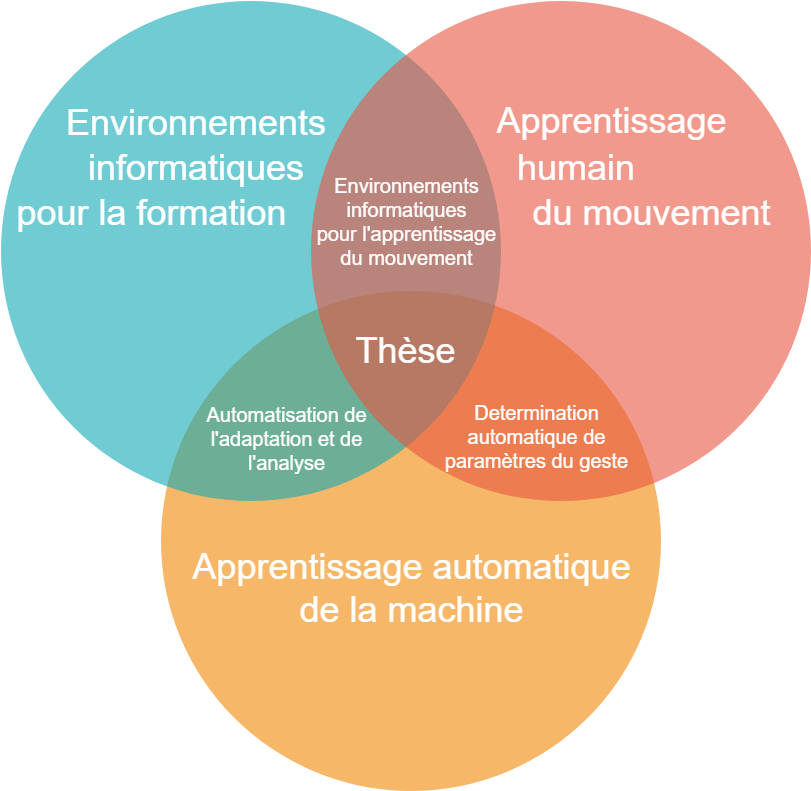
\includegraphics[scale=0.25]{img/cadre.png}
	\end{frame}
	
	\begin{frame}{\secname}
	\centering
		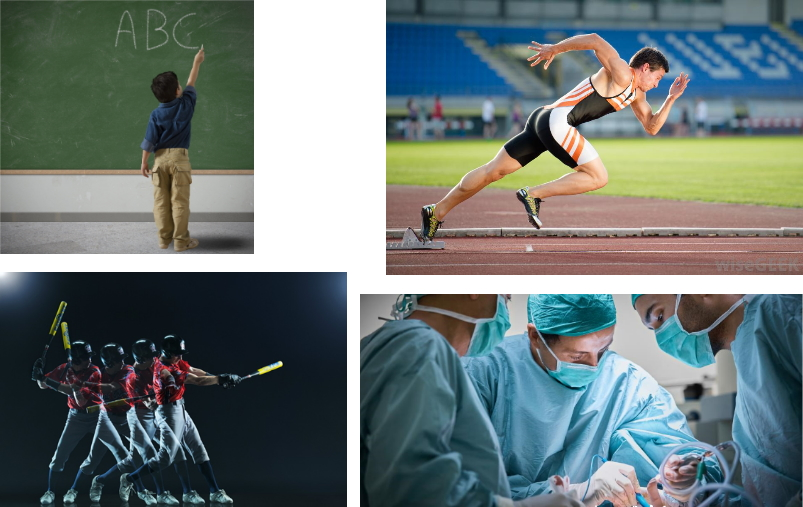
\includegraphics[scale=0.5]{img/motion_in_general.jpg}
	\end{frame}

	\begin{frame}{\secname}
	    \begin{block}{EIAH \mycite{Tchounikine2009PdR}}
	    « Environnements ayant pour but de favoriser l'apprentissage, en aidant, guidant et évaluant les apprenants d'une part et en assistant les enseignants d'autre part : que ce soit en présentiel, à distance, ou en situation mixte. »
	    \end{block}

	\begin{block}{Apprentissage du mouvement}
		 Apprentissage d'une succession de postures d'un corps dans l'espace, ayant une ou plusieurs finalités : le geste lui-même (caractère moteur), l'objectif du geste (caractère fonctionnel) ou les connaissances du sujet (caractère structurant)
	\end{block}
		
		\begin{block}{Apprentissage automatique}
		Plusieurs familles d'algorithmes d'apprentissage automatique : Apprentissage supervisé / non-supervisé / semi-supervisé
		\end{block}
	\end{frame}
	
	\subsection{Problématique de la thèse}
	\begin{frame}{Problématique}
		Quels sont les facteurs limitant à la réalisation d'un EIAH dédié à l'apprentissage humain de gestes, qui prend en compte les besoins d'observation et d'analyse de l'expert ?\\
		
		\vspace{1cm}		
		
		4 verrous identifiés :
		\begin{itemize}[label=$\bullet$]
			\item Détermination des propriétés du mouvements
			\item Formalisation de l'expertise
			\item Visualisation d'indicateurs intelligibles
			\item Restitution adaptée sous forme de conseils
		\end{itemize}
	\end{frame}
	
	
	\section{État de l'art}
	\subsection{EIAH pour l'apprentissage du geste}
		
	\begin{frame}{\secname}
		\centering
		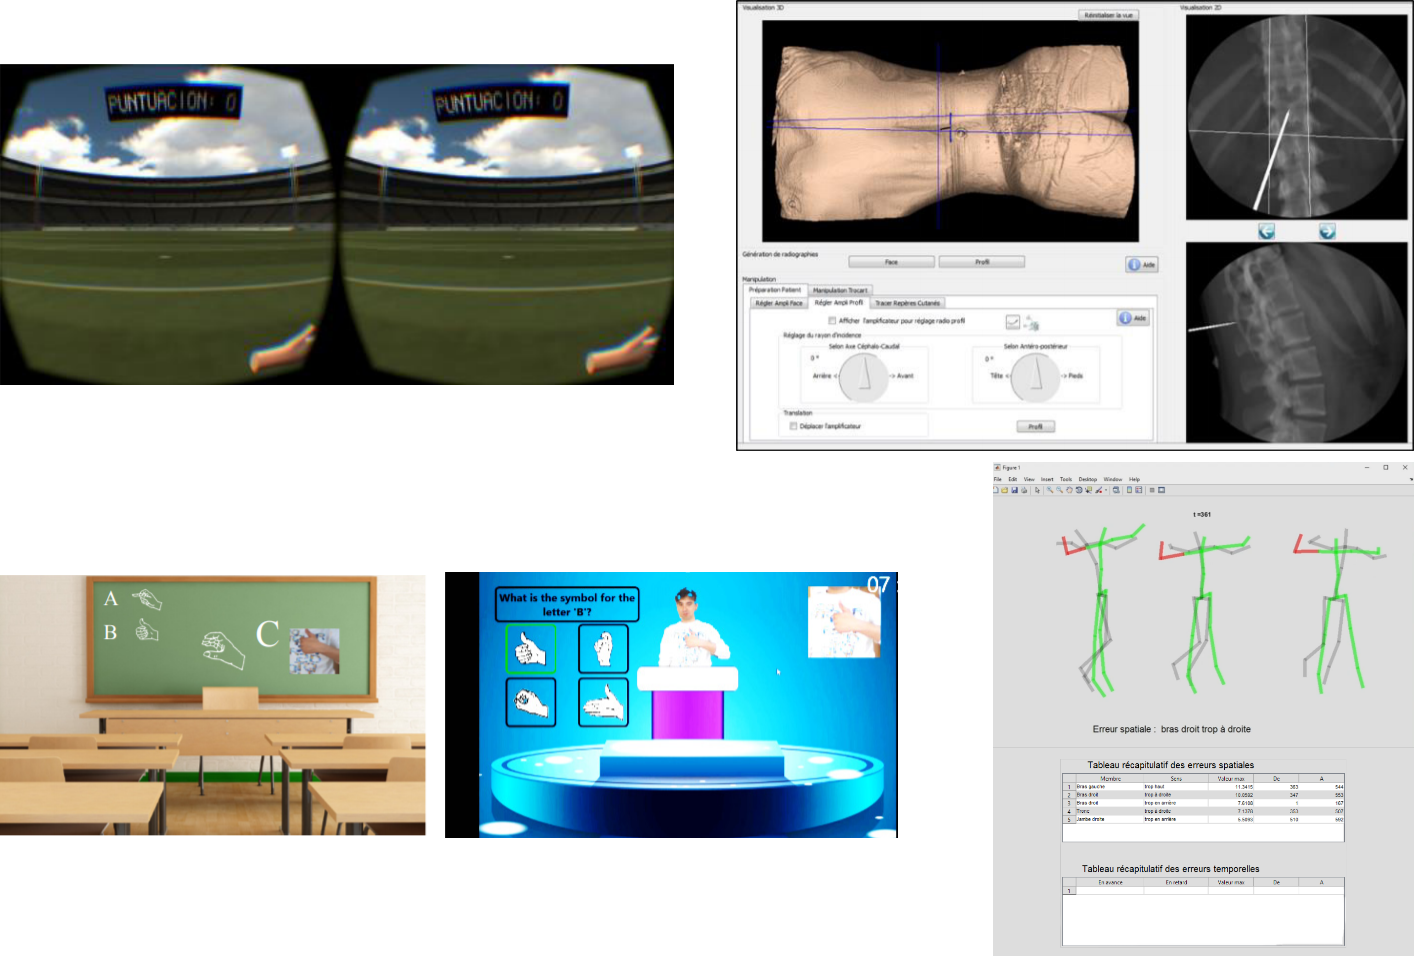
\includegraphics[scale=0.35]{img/all_eiah.png}
	\end{frame}
	
	\begin{frame}{Limites récurrentes}
		\centering
		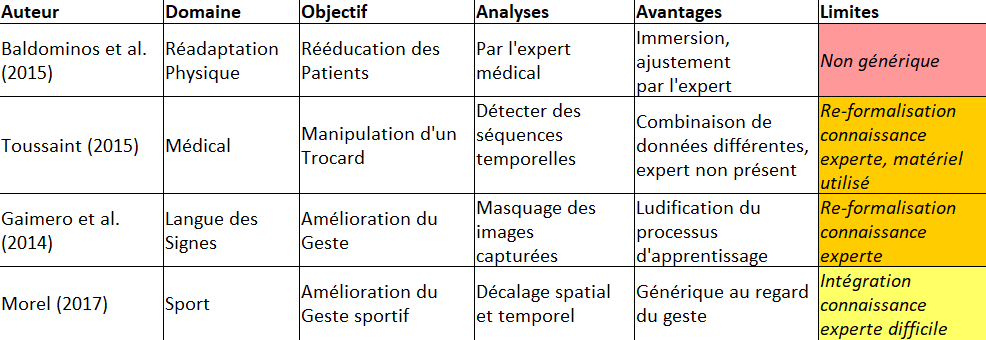
\includegraphics[scale=0.43]{img/tableau_eiah_5.png}
	\end{frame}
	
	\subsection{Analyse du mouvement capturé}
	\subsubsection{Descripteurs du mouvement}
	\begin{frame}{\subsubsecname}
		\begin{block}{Descripteur du mouvement}
			Un descripteur est un indicateur calculé à partir du mouvement brut :  « Des observables signifiant sur le plan pédagogique » calculés à partir de traces (tous types de données, générées à partir des interactions de l’étudiant avec le système) ou d’autres indicateurs \mycite{Choquet2007MTf}
		\end{block}
	\end{frame}
	
	\subsubsection{Analyse par observation humaine}
	\begin{frame}{\subsubsecname}
		\begin{itemize}[label=$\bullet$]
			\item Visualisation de la performance de l'apprenant \mycite{Burns2011Uvh}
			\item Superposition de l'apprenant à un ou des modèles expert \mycite{Yoshinaga2015Doa}
		\end{itemize}
		\centering
			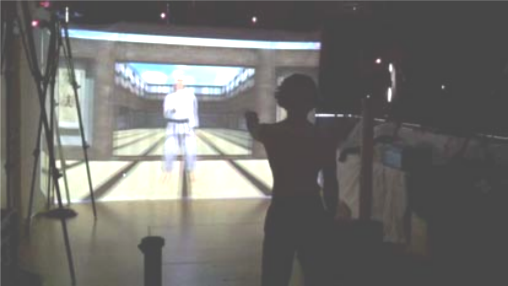
\includegraphics[scale=0.4]{img/Burns_karate.png}
			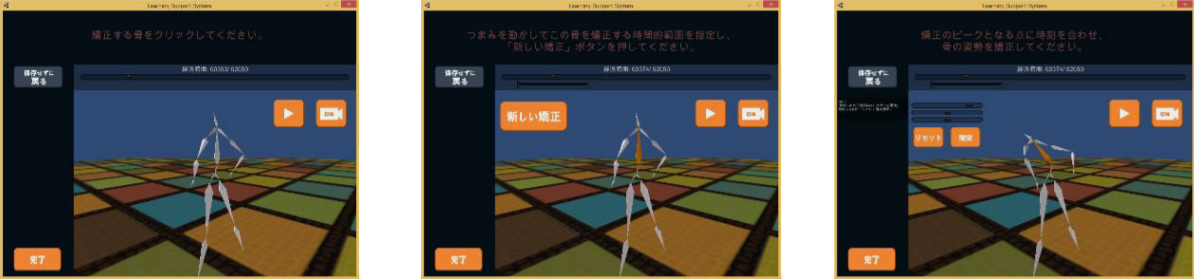
\includegraphics[scale=0.4]{img/Yoshiniga_archery.png}
	\end{frame}
	
	\subsubsection{Analyse par observation d'indicateurs}
	\begin{frame}{\subsubsecname}
		\begin{itemize}[label=$\bullet$]
			\item Positions relatives des parties du corps à des moments clés du lancer \mycite{Yamaoka2013FoF}
			\item Décomposition du mouvement à l'aide d'un seul descripteur \mycite{Kyan2015ABD}
			
			\centering
				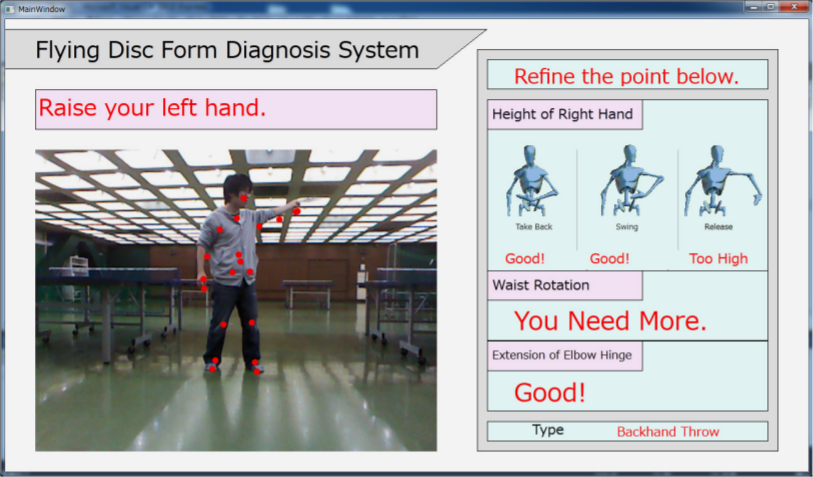
\includegraphics[scale=0.3]{img/flying_disc_TEL.png}
				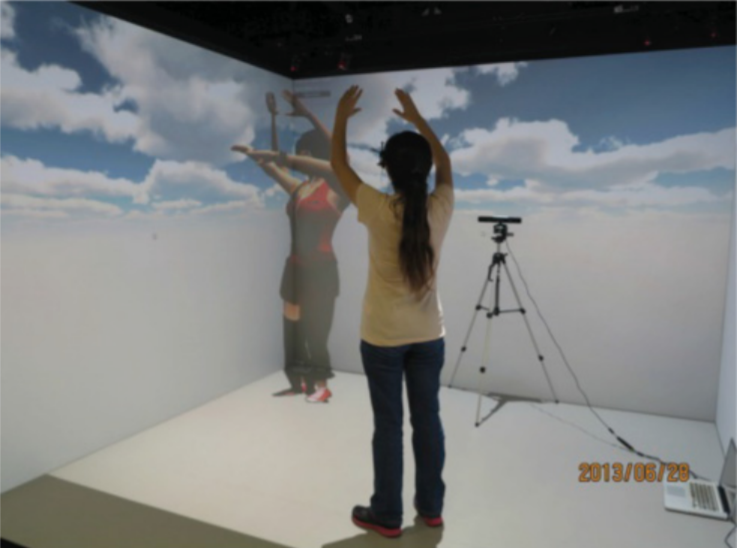
\includegraphics[scale=0.3]{img/dance_cave_TEL.png}
		\end{itemize}
		
				
	\end{frame}
	
	\subsubsection{Analyse par détection de séquence ordonnée d'actions}
	\begin{frame}{\subsubsecname}
		\begin{itemize}[label=$\bullet$]
			\item Scénarisation par l'expert, puis reproduction par l'apprenant \mycite{Baudouin2007, Mahdi2019TaE}	
			
			\vspace{1cm}
			
			\centering
				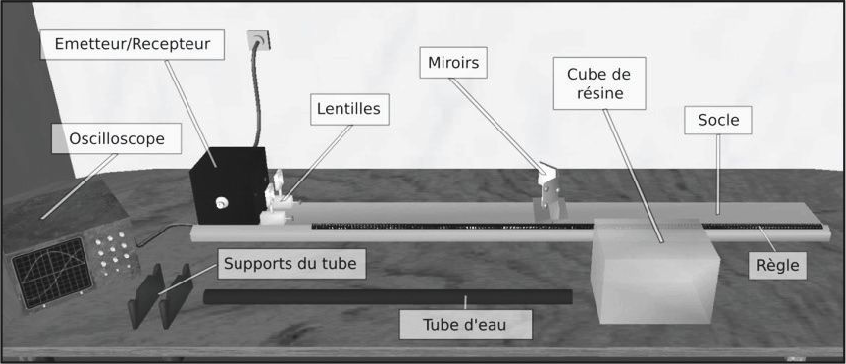
\includegraphics[scale=0.4]{img/eiah_baudouin.png}
		\end{itemize}
	\end{frame}
	
	\subsubsection{Analyse basée sur des techniques d'apprentissage automatique}
	\begin{frame}{\subsubsecname}
		\begin{itemize}[label=$\bullet$]
			\item Évaluation de gestes sans \textit{a priori} sur le geste en lui-même \mycite{Pirsiavash2014AQA})
			\item Segmentation, reconnaissance et évaluation de gestes à l'aide d'algorithmes de logique floue \mycite{Patrona2018MaA})
		\end{itemize}
		
		\centering
		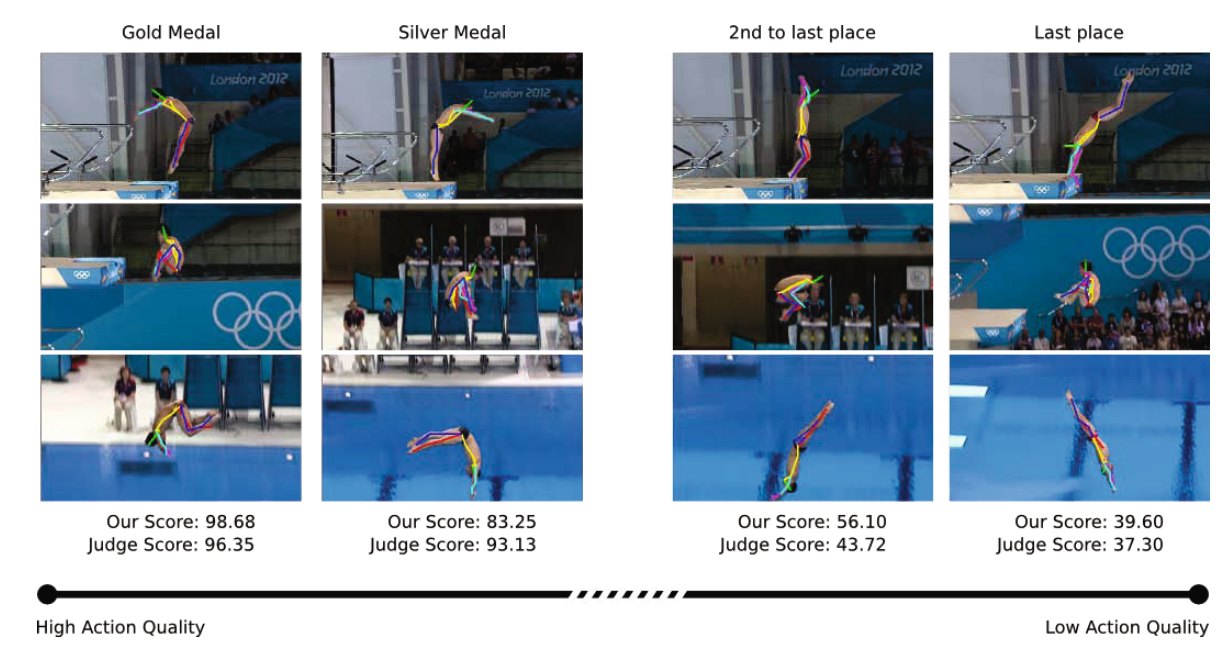
\includegraphics[scale=0.3]{img/olympic_games.png}
	\end{frame}
	
	\subsubsection{Bilan des systèmes existants}
	\begin{frame}{\subsubsecname}
		\begin{table}[]
			\resizebox{\textwidth}{!}{%
			\begin{tabular}{c|c|c|c}
			\textbf{Système basé sur...} & \textbf{Place de l'utilisateur} & \textbf{Objectif} & \textbf{Inconvénients} \\\hline
			Analyse humaine & Au centre & \makecell{Fournir des visualisations\\du geste} & \textit{\makecell{Difficulté pour non-expert,\\pas d'analyse}} \\\hline
			Descripteurs & Variable & \makecell{Fournir des valeurs\\pertinentes} & \textit{\makecell{Nécessite des\\connaissances scientifiques}} \\\hline
			Séquence d'actions & Variable & \makecell{Segmenter et analyser\\le mouvement} & \textit{\makecell{Intégration de la connaissance\\ lors de la conception}} \\\hline
			Analyse automatique & Souvent écarté & \makecell{Analyser le geste\\sans présence d'expert} & \textit{Absence de l'expert} \\
			\end{tabular}
			}
		\end{table}
	\end{frame}
	
	\subsection{Positionnement}
	\begin{frame}{\subsecname}
		\begin{itemize}[label=$\bullet$]
			\item Assistance à l'expert dans sa tâche d'analyse
			\item Système d'évaluation du geste, proposant également des indicateurs visuels
			\item Intégration de la connaissance experte avant l'utilisation en situation d'apprentissage, sans nécessité de ré-ingénierie
		\end{itemize}
	\end{frame}
	
	\subsection{Questions de recherche}
	\begin{frame}{\subsecname}
		\begin{itemize}[label=$-$]
			\item \textbf{Q1} : Est-il possible de développer un système permettant de caractériser le geste à l'aide de l'intégration de l'expertise d'un enseignant?
			\item \textbf{Q2} : Comment évaluer et comparer le geste (ou ses propriétés) de l'apprenant avec celui de l'enseignant afin d'évaluer la progression de l'apprentissage?
			\item \textbf{Q3} : Comment, dans une situation d'apprentissage de gestes donnée, proposer des retours pertinents et compréhensibles aux acteurs de l'apprentissage non spécialistes en analyse du mouvement?
		\end{itemize}
	\end{frame}

	\section{Système MLA}
	\subsection{Motion Learning Analytics}
	\begin{frame}{\subsecname}
		\begin{block}{Motion Learning Analytics (MLA)}
			\begin{itemize}[label=$\bullet$]
				\item Propose un ensemble d'outils pour pré-traiter et extraire des informations permettant d'analyser un geste
				\item Permet également de comparer les mouvements à ceux d'un expert, à l'aide de techniques de clustering
				\item Propose un ensemble de métriques, ainsi que de visualisation pour assister l'expert dans sa tâche d'évaluation des gestes
			\end{itemize}
		\end{block}
	\end{frame}
	
	\subsubsection{Architecture MLA}
	\begin{frame}{\subsubsecname}
	\centering
		\includegraphics[scale=0.3]{img/mla/MLA_color_1.png}
	\end{frame}

	\nonumberingframe{\subsubsecname}
	\centering
		\includegraphics[scale=0.3]{img/mla/MLA_color_2.png}
	\end{frame}

	\nonumberingframe{\subsubsecname}
	\centering
		\includegraphics[scale=0.3]{img/mla/MLA_color_3.png}
	\end{frame}

	\nonumberingframe{\subsubsecname}
	\centering
		\includegraphics[scale=0.3]{img/mla/MLA_color_4.png}
	\end{frame}

	\nonumberingframe{\subsubsecname}
	\centering
		\includegraphics[scale=0.3]{img/mla/MLA_color_5.png}
	\end{frame}

	\nonumberingframe{\subsubsecname}
	\centering
		\includegraphics[scale=0.3]{img/mla/MLA_color_6.png}
	\end{frame}

	\nonumberingframe{\subsubsecname}
	\centering
		\includegraphics[scale=0.3]{img/mla/MLA_color_7.png}
	\end{frame}

	\nonumberingframe{\subsubsecname}
	\centering
		\includegraphics[scale=0.3]{img/mla/MLA_color_8.png}
	\end{frame}

	\nonumberingframe{\subsubsecname}
	\centering
		\includegraphics[scale=0.3]{img/mla/MLA_color_9.png}
	\end{frame}

	\nonumberingframe{\subsubsecname}
	\centering
		\includegraphics[scale=0.3]{img/mla/MLA_color_10.png}
	\end{frame}

	\nonumberingframe{\subsubsecname}
	\centering
		\includegraphics[scale=0.3]{img/mla/MLA_color_11.png}
	\end{frame}

	\nonumberingframe{\subsubsecname}
	\centering
		\includegraphics[scale=0.3]{img/mla/MLA_color_12.png}
	\end{frame}

	\nonumberingframe{\subsubsecname}
	\centering
		\includegraphics[scale=0.3]{img/mla/MLA_color_13.png}
	\end{frame}

	\nonumberingframe{\subsubsecname}
	\centering
		\includegraphics[scale=0.3]{img/mla/MLA_color_14.png}
	\end{frame}

	\nonumberingframe{\subsubsecname}
	\centering
		\includegraphics[scale=0.3]{img/mla/MLA_color_15.png}
	\end{frame}

	\nonumberingframe{\subsubsecname}
	\centering
		\includegraphics[scale=0.3]{img/mla/MLA_color_16.png}
	\end{frame}
	
	\begin{frame}{Aspects techniques}
		\begin{itemize}[label=$\bullet$]
			\item Pré-traitements / extractions de descripteurs :
			\begin{itemize}[label=$-$]
				\item C++
				\item OpenGL, GLM, Glew, SDL, json
			\end{itemize}
			\item Analyse automatique et retours à l'apprenant : 
			\begin{itemize}[label=$-$]
				\item Python
				\item pyQT, sklearn
			\end{itemize}
		\end{itemize}		
		\vspace{1cm}
		
		Représentation du mouvement au sein du système :
		\centering
		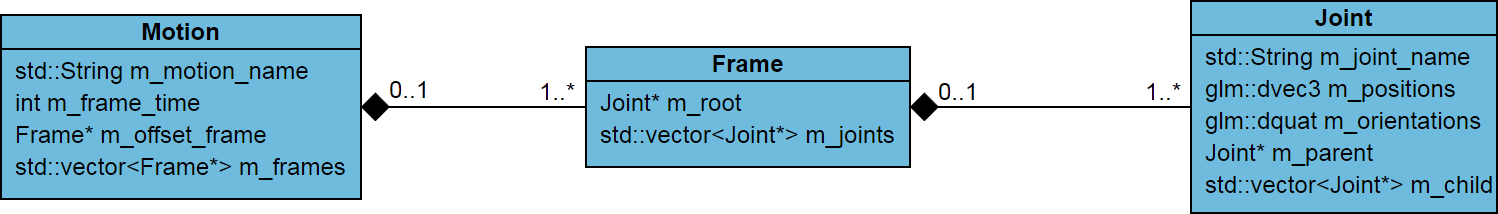
\includegraphics[scale=0.35]{img/class_diagram_motion_MLA.png}
		%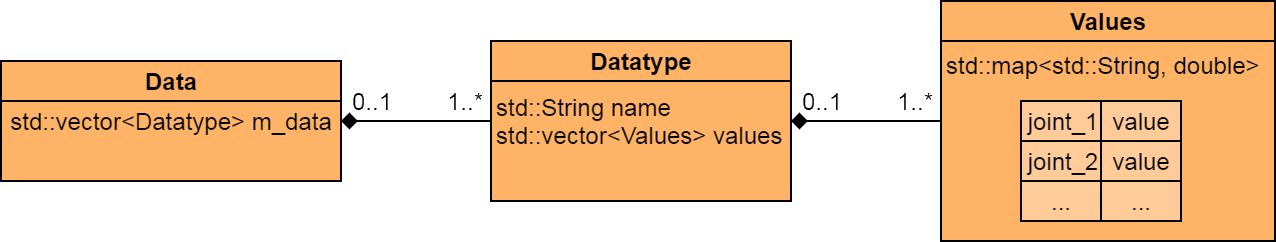
\includegraphics[scale=0.30]{img/class_diagram_datatype_MLA.png}
	\end{frame}

	\subsection{Traitements des données}
	
	\subsubsection{Matériel de capture}
	\begin{frame}{Perception Neuron}
		\centering
		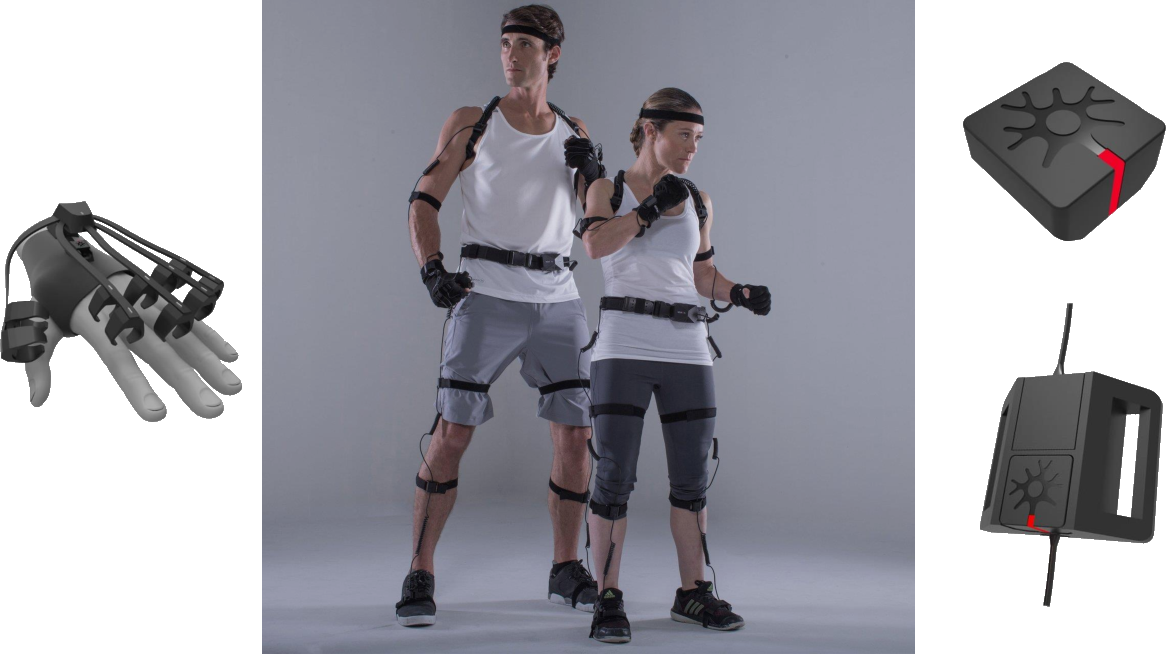
\includegraphics[scale=0.4]{img/Perception_Neuron.png}
	\end{frame}
	
	\subsubsection{Pré-traitements}
	\begin{frame}{Pré-traitements \mycite{couland:hal-02002381}}
		\begin{block}{Variation de la taille des membres}
			Fixation de la taille des membres à l'aide de la posture de référence (posture à l'indice 0)
		\end{block}
		
	\begin{block}{Filtrage et extraction du moment d'intérêt}
		\centering
			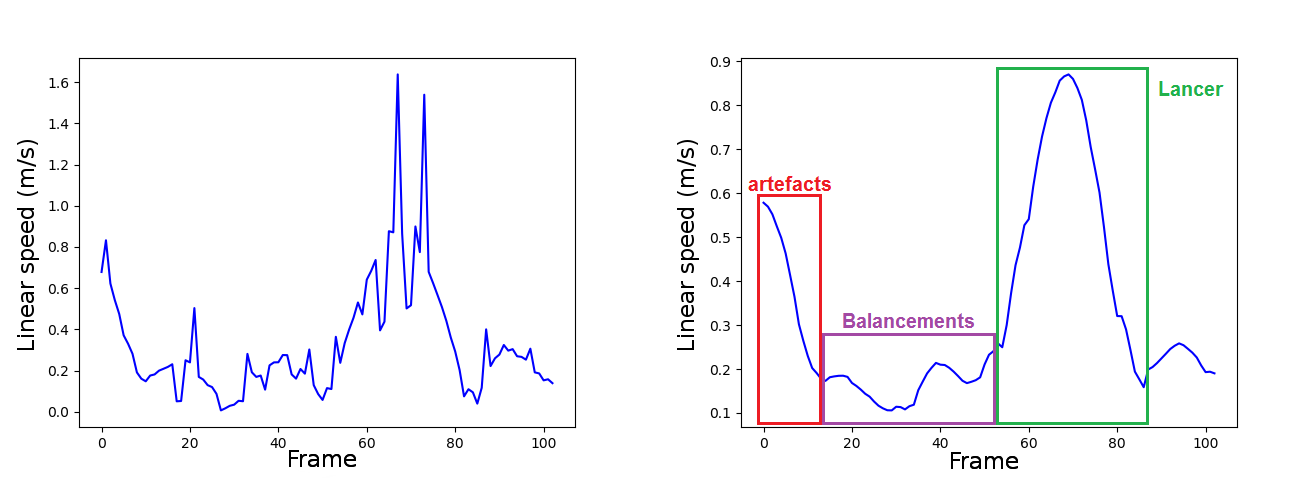
\includegraphics[scale=0.35]{img/before_after_savgol_complete.png}
	\end{block}
		
	\end{frame}
	
	\subsection{Analyse et représentation visuelle}
	\begin{frame}{\subsecname}
	Objectif : assister l'expert dans sa tâche d'évaluation du geste, en lui permettant d'obtenir un retour visuel sur les différences entre le geste de l'apprenant et le sien.
	Pré-requis :
	\begin{itemize}[label=$\bullet$]
		\item Données de l'expert réparties en bons gestes / gestes correspondant à un défaut
		\item Données de l'apprenant
		\item Liste de descripteurs à associer aux défauts
	\end{itemize}
	\end{frame}
	
	\begin{frame}{Méthode}
	\begin{itemize}
		\item \textbf{1.} Normalisation des données
		\item \textbf{2.} Clustering des données de l'expert à l'aide d'un k-means, afin d'obtenir deux groupes correspondant aux bons et aux mauvais gestes (apprentissage semi-supervisé)
		\item \textbf{3.} Comparaison des données de l'apprenant à celles de l'expert (distance euclidienne)
		\item \textbf{4.} Retour sous forme visuelle (utilisation d'un PCA si dimensionnalité des données > 2)
	\end{itemize}
	
	\end{frame}
	
	\begin{frame}{Étape de clustering}
	\centering
		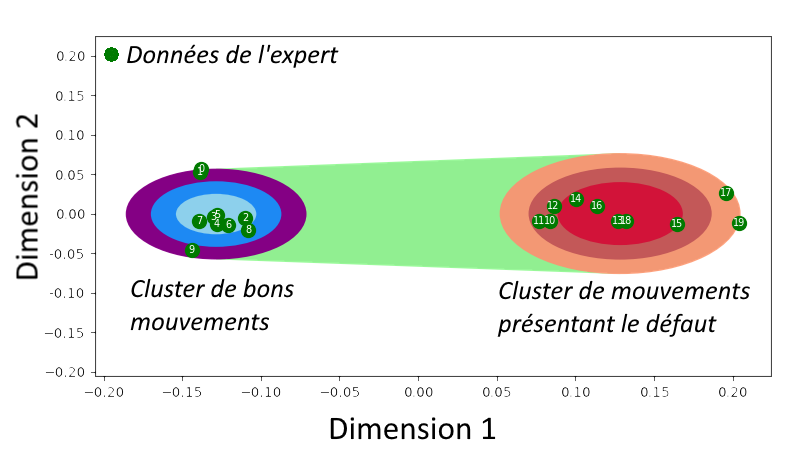
\includegraphics[scale=0.65]{img/feedback_expert_cluster_example.png}
	\end{frame}
	
	\begin{frame}{Étape de comparaison}
	\centering
		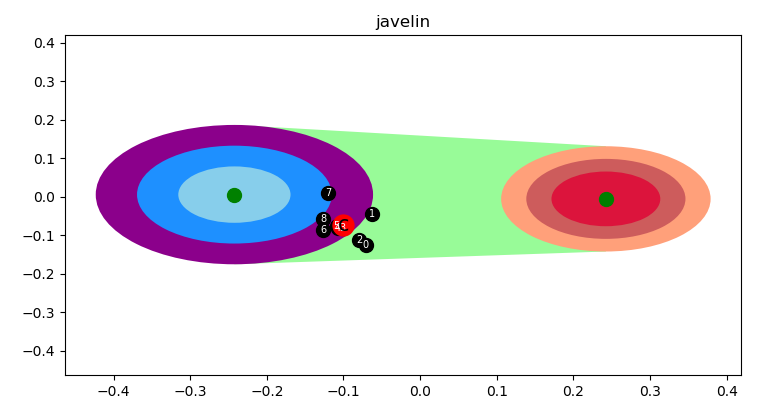
\includegraphics[scale=0.53]{img/feedback_one.png}
	\end{frame}


	\section{Expérimentations}
	\subsection{Hypothèses en lien avec les expérimentations}
	\begin{frame}{\subsecname}
		\begin{itemize}[label=$-$]
			\item \textbf{H1} : regrouper les gestes selon leurs propriétés cinématiques communes
			\item \textbf{H2} : séparer les gestes des apprenants en deux groupes correspondant à une dichotomie geste réussi / geste raté
			\item \textbf{H3} : séparer les gestes en fonction de propriétés attendues et identifiées par l'expert
			\item \textbf{H4} : corriger chaque défaut du geste de l'apprenant, en lui indiquant les défauts majeurs à corriger en premier
			\item \textbf{H5} : améliorer l'apprentissage du geste par rapport à une situation sans le système MLA
			\item \textbf{H6} : améliorer l'apprentissage du geste par rapport à une situation sans MLA, et à une situation avec MLA et sans enseignant
		\end{itemize}
	\end{frame}

	\subsection{Protocole commun}
	\begin{frame}{Protocole commun aux trois expérimentations}
		\begin{itemize}[label=$\bullet$]
			\item Instructions données à l'apprenant
			\item Mesure selon les préconisations de NOITOM
			\item Calibrations de la combinaison d'acquisition de mouvement
			\item Familiarisation avec la combinaison 
		\end{itemize}
	
		\centering
		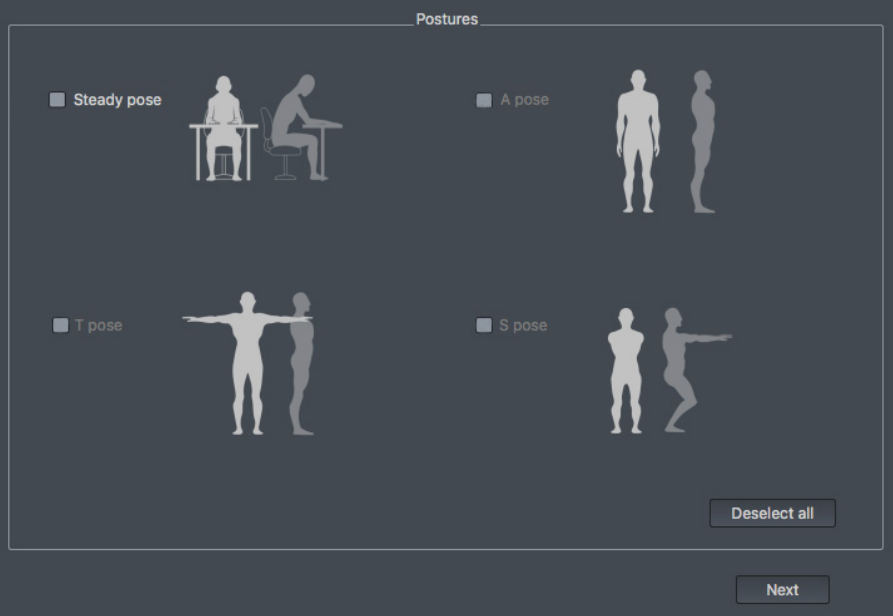
\includegraphics[scale=0.3]{img/percpetion_neuron_calibrations.png}
	\end{frame}
	
	\subsubsection{Workflow du système MLA}
	\begin{frame}{\subsubsecname}
	\centering
		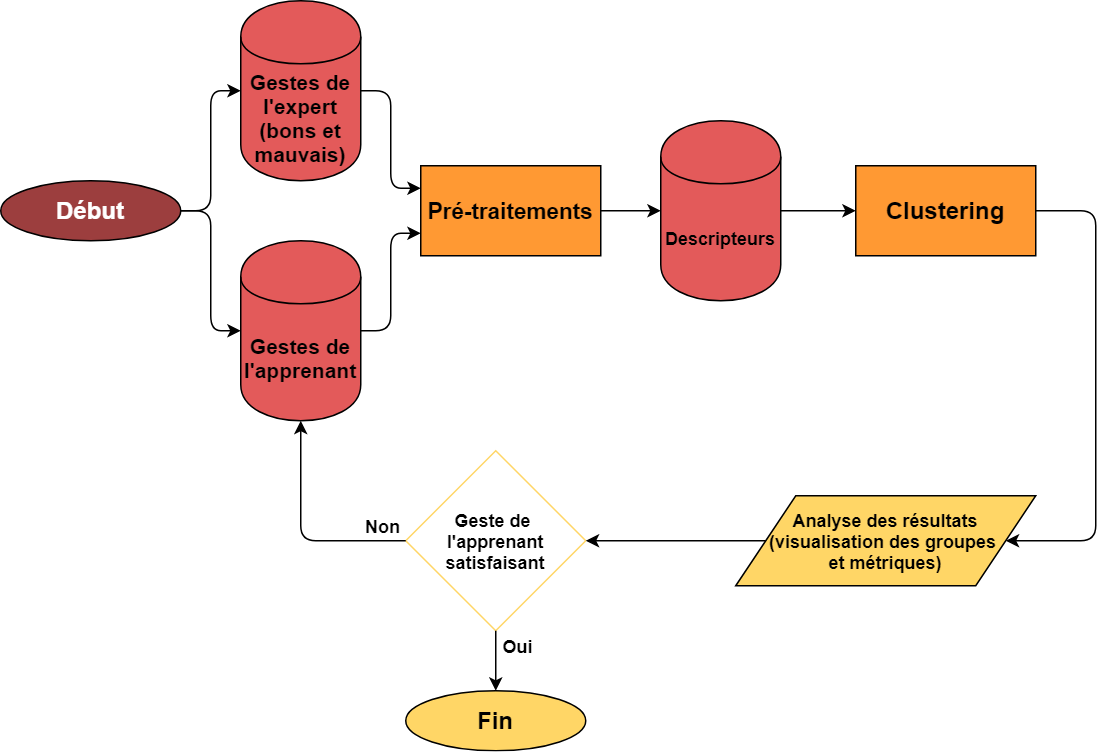
\includegraphics[scale=0.25]{img/workflow_MLA.png}
	\end{frame}
	
	\subsubsection{Métriques calculées}
	\begin{frame}{\subsubsecname : Average Silhouette Score (\textit{ASS})}
		\begin{block}{Silhouette Score}
			Calcule la bonne appartenance d'un point au cluster qui lui est assigné, en calculant la distance de ce point à tous les autres contenus dans le même cluster par rapport à ceux des autres clusters.
		\end{block}
		
		\begin{block}{Average Silhouette Score \mycite{Rousseeuw1987Sag}}
			Moyenne des Silhouette Scores de chaque point de donnée.
		\end{block}
	\end{frame}
	
	\begin{frame}{Average Silhouette Score (\textit{ASS})}
		\begin{itemize}[label=$\bullet$]
			\item $[0;0.25]$ : aucune structure n'est discernable au sein des données
			\item$ ]0.25; 0.5]$ : il existe une structure, bien que mal définie, voire artificielle
			\item $]0.5;0.70
			]$ : une structure existe au sein des données (séparation correcte des clusters)
			\item $]0.7;1]$ : une structure est clairement définie au sein des données (très bonne séparation des clusters)
		\end{itemize}
	\end{frame}
	
	\begin{frame}{\subsubsecname : Adjusted Rand Index (\textit{ARI})}
		\begin{block}{Adjusted Rand Index \mycite{Morey1984ARI}}
			Mesure de similarité entre deux partitionnements de données différents. Cette mesure est un ajustement du Rand Index \mycite{Rand2971RI}. Une valeur de 1 indique une correspondance parfaite entre les deux partitionnement, alors qu'une valeur de 0 indique une affectation aléatoire des données. La normalisation induite par l'ajustement peut produire des valeurs négatives \mycite{Meila2007Cca}. 
		\end{block}
	\end{frame}
	
	\begin{frame}{Trois expérimentations}
		\begin{itemize}[label=$\bullet$]
			\item Lancer de balles et Bottle Flip Challenge
			
			\begin{itemize}[label=$-$]
				\item Validation du processus complet
				\item Chaîne de traitement
				\item Analyse automatique
			\end{itemize}
			
			\item Lancer de fléchettes
			\begin{itemize}[label=$-$]
				\item Test du système en condition réelles
				\item Retour à l'apprenant
			\end{itemize}
			
		\end{itemize}		
	\end{frame}

	\subsection{Lancer de balle}
	\subsubsection{Objectifs et principe}
	\begin{frame}{\subsecname : \MakeLowercase{\subsubsecname}}
		\begin{block}{Objectif}
			Vérifier si le système est capable de séparer les gestes selon un étiquetage vérifiable par un humain à l'aide des descripteurs et des algorithmes choisis (\textbf{H1}, \textbf{H2}).
		\end{block}
		
		\vspace{1cm}
		
		\centering
		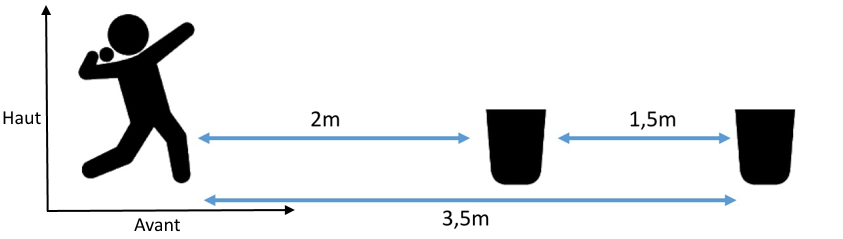
\includegraphics[scale=0.5]{img/ball_throwing.png}

	\end{frame}
	
	\subsubsection{Résultats}
	\begin{frame}{\subsecname : \MakeLowercase{\subsubsecname}}
		\begin{block}{Participants}
			\begin{itemize}[label=$\bullet$]
				\item 2 participants
				\item 100 lancers par personne
			\end{itemize}
		\end{block}
		
	Algorithme utilisé : k-means, avec $k=2$.
	\begin{itemize}
		\item Séparation correcte des clusters (norme du vecteur vitesse de la main et vecteurs vitesses en x, y et z ($ASS \approx 0.6$)) / \textbf{H1} validée dans le contexte de cette expérimentation
		\item Séparation correspondant à l'étiquetage « type de lancer » ($ARI \approx 0.85$)
		\item Séparation ne correspondant pas au degré de réussite du geste : \textbf{H2} non validée
	\end{itemize}
		
		
	\end{frame}


	\subsection{Bottle Flip Challenge}
	\subsubsection{Objectifs et principe}
	\begin{frame}{\subsecname : \MakeLowercase{\subsubsecname}}
		\begin{block}{Objectif}
			 Déterminer s'il est possible d'obtenir une séparation des données en deux clusters, correspondant au degré de réussite du geste. (\textbf{H2}).
		\end{block}
	
		\centering
		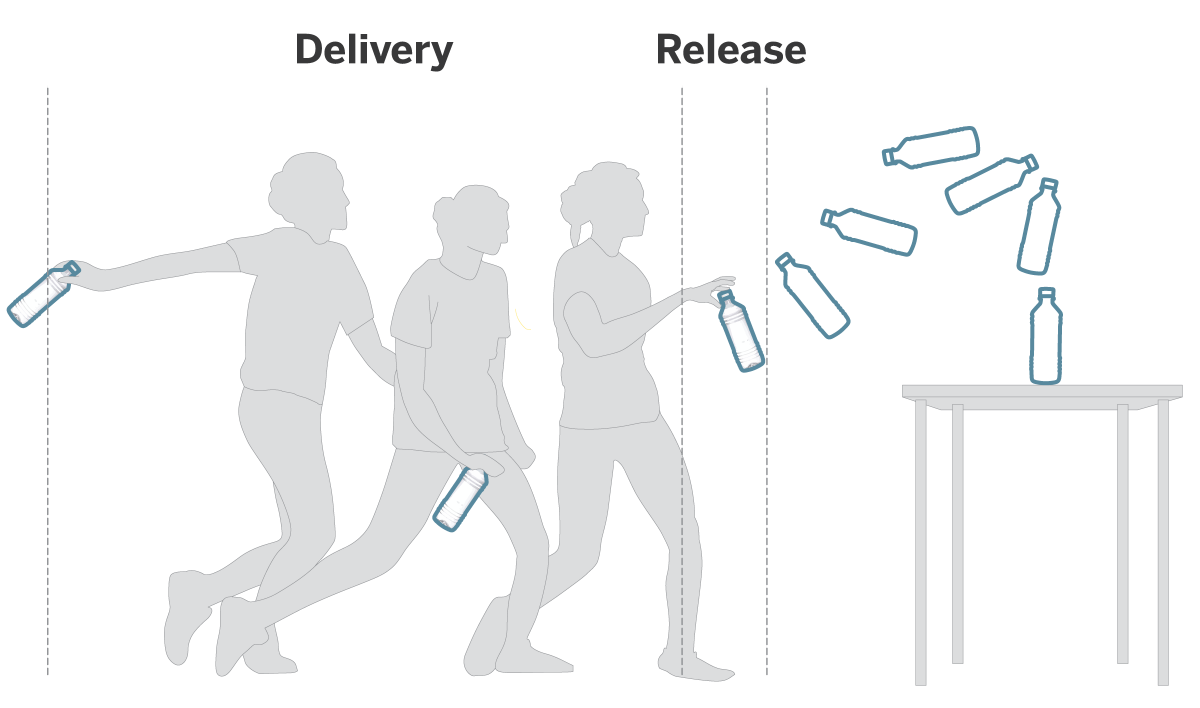
\includegraphics[scale=0.2]{img/BFC_example.png}
	\end{frame}
	
	\subsubsection{Résultats}
	\begin{frame}{\subsecname : \MakeLowercase{\subsubsecname}}
		\begin{block}{Participants}
			\begin{itemize}[label=$\bullet$]
				\item 13 participants (2 gauchers, 11 droitiers)
				\item 100 lancers par personne
			\end{itemize}
		\end{block}

		Algorithme utilisé : k-means, avec $k=2$.
		\begin{itemize}
			\item Séparation correcte des clusters pour les vecteurs vitesse en x, y et z des droitiers ($ASS \approx 0.75$)
			\item Séparation ne correspondant pas au degré de réussite du geste ($ARI \approx 0$): \textbf{H2} non validée
		\end{itemize}
		
	\end{frame}

	\subsection{Lancer de fléchettes}
	\subsubsection{Objectifs et principe}
	\begin{frame}{\subsecname : \MakeLowercase{\subsubsecname}}
		\begin{block}{Objectifs}
			\begin{itemize}[label=$\bullet$]
				\item Montrer qu'il est possible de donner des conseils pertinents lors de la réalisation des gestes (\textbf{H3}, \textbf{H4})
			 	\item Montrer qu'une amélioration du geste résultait de ces conseils (\textbf{H5})
			 	\item Évaluation en terme d'usage de l'efficacité du système selon les modalités précédemment citées (\textbf{H6})
			 \end{itemize}
		\end{block}
	
		\begin{block}{Domaine applicatif}
			Lancer de fléchettes
		\end{block}
		
	\end{frame}
	
	\subsubsection{Position de tir}
	\begin{frame}{\subsecname : \MakeLowercase{\subsubsecname}}
		\centering
		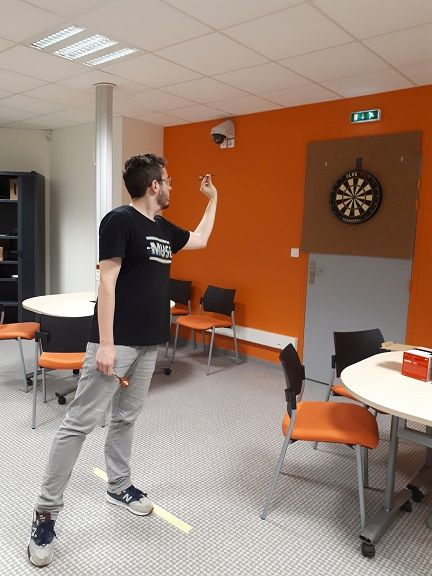
\includegraphics[scale=0.3]{img/darts_position_alt.jpg}
	\end{frame}
	
	\subsubsection{Acquisition des données de l'expert et participants}
	\begin{frame}{\subsecname : \subsubsecname}
		\begin{block}{Acquisition des données de l'expert}
			\begin{itemize}
				\item \textbf{1.} Identification des défauts quantifiables
				\item \textbf{2.} Capture de mouvements de lancers corrects réalisés par l'expert
				\item \textbf{3.} Pour chaque défaut, capture de mouvements de lancers par l'expert présentant ce défaut 
			\end{itemize}
		\end{block}
	
		\begin{block}{Participants}
			\begin{itemize}[label=$\bullet$]
				\item 45 participants, répartis en 3 groupes de 15 personnes :
				\begin{itemize}
					\item \textbf{Groupe 1} : Conseils de l'expert seulement
					\item \textbf{Groupe 2} : Conseils du système seulement
					\item \textbf{Groupe 3} : Expert s'appuyant sur le système pour donner ses conseils
				\end{itemize}
				\item 36 lancers par personne ($4 \times 9$ lancers)
			\end{itemize}
		\end{block}
	\end{frame}
	
	\begin{frame}{Exemple de lancer}
	\centering
%		\includemedia[
%  			activate=pageopen,
%  			width=274pt,height=154pt,
%			addresource=img/darts_throwing_2.mp4,
%			flashvars={%
%     			source=img/darts_throwing_2.mp4% same path as in addresource!
%				&autoPlay=true
%				&loop=true
%  			}  
%		]{}{VPlayer.swf}
	%\includemovie[controls,poster]{10cm}{5cm}{img/darts_throwing_2.mp4}
	\href{run:img/darts_throwing_2.mp4}{Vidéo de démonstration ici}
	\end{frame}
	
	\begin{frame}{Visualisation d'une série}
		\centering
		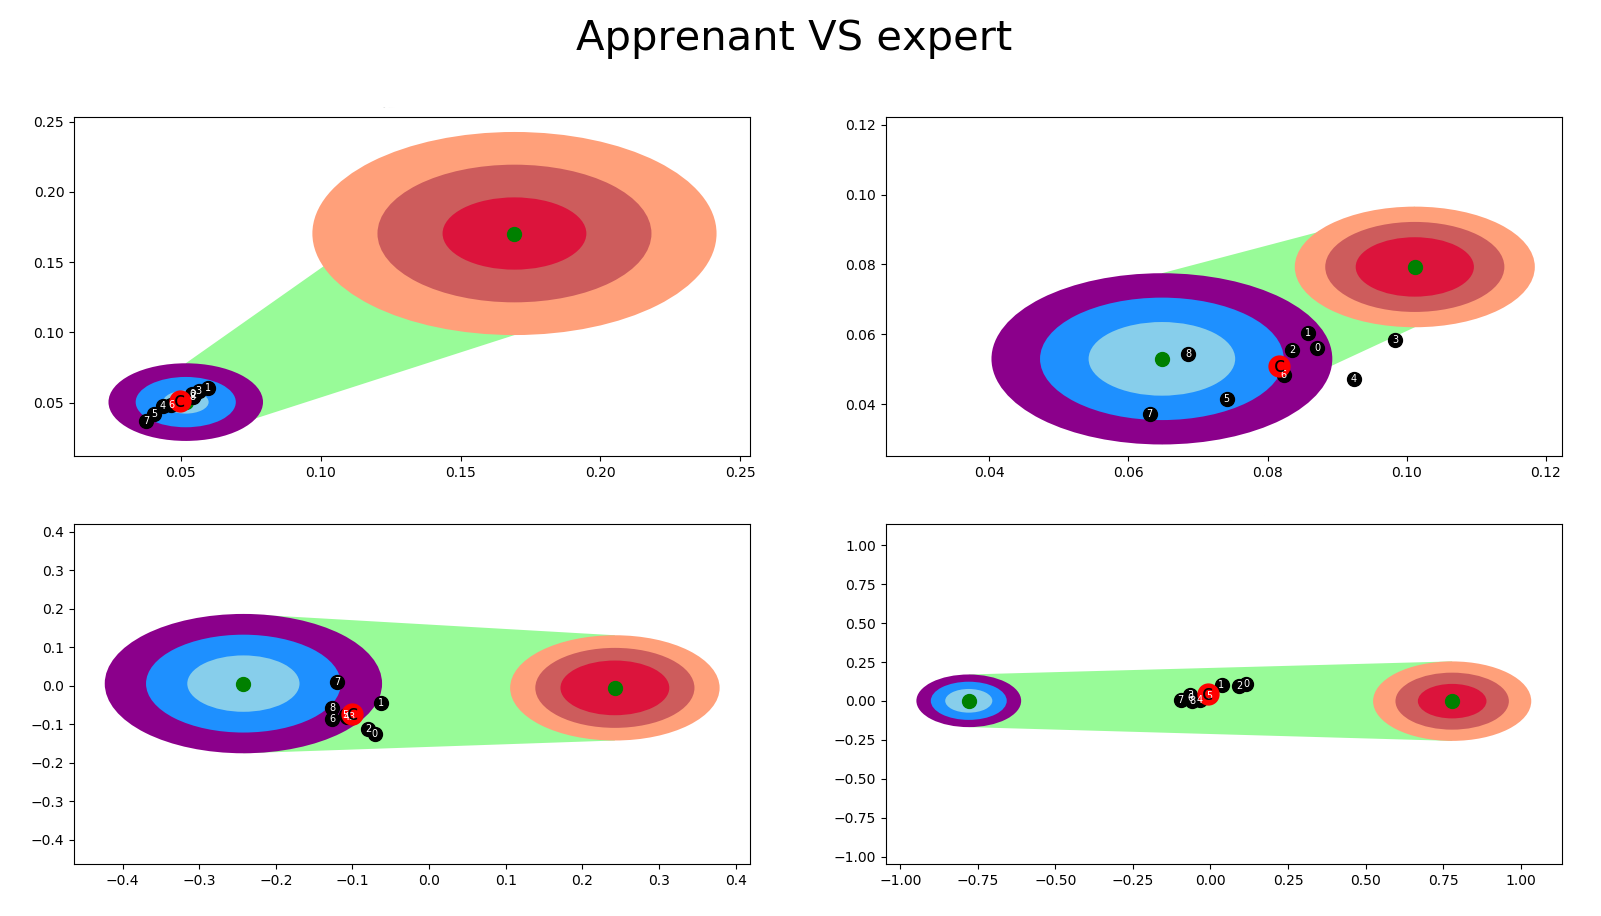
\includegraphics[scale=0.27]{img/feedback_grp_example.png}
	\end{frame}
	
	\begin{frame}{Visualisation de la progression}
		\centering
		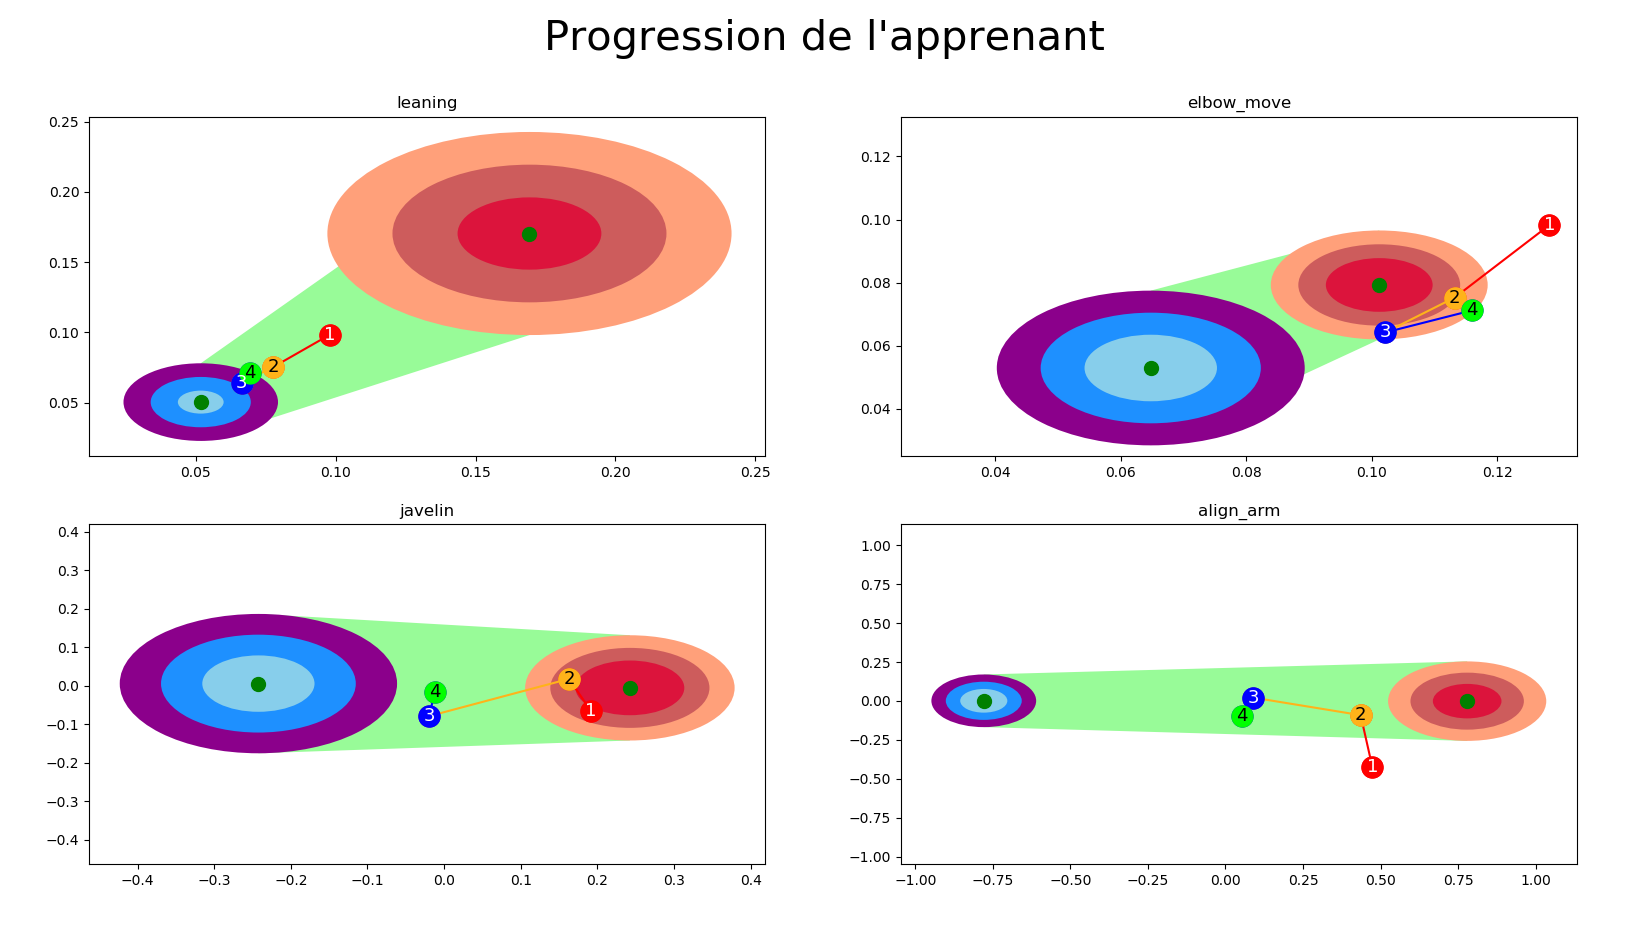
\includegraphics[scale=0.27]{img/progression.png}
	\end{frame}
	
	\subsubsection{Défauts}
	\begin{frame}{\subsubsecname}
		\centering
		\begin{table}
		\resizebox{10cm}{!}{%
			\begin{tabular}{cc}
			Corps penché (\textit{leaning)} & Mouvement du coude (\textit{elbow move})\\
				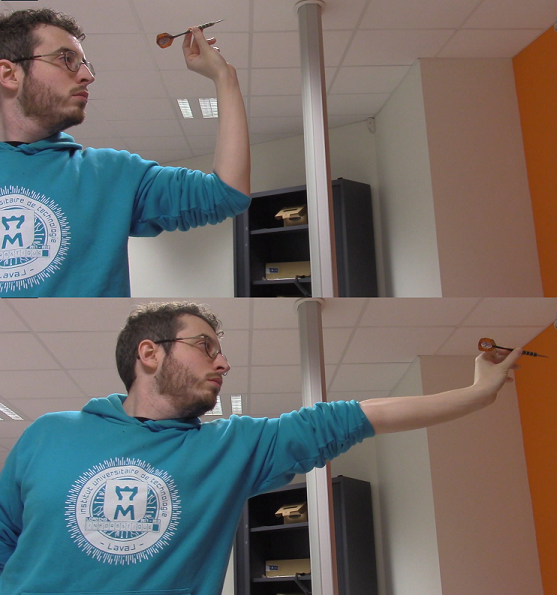
\includegraphics[scale=0.25]{img/darts_leaning_final.png} & 
				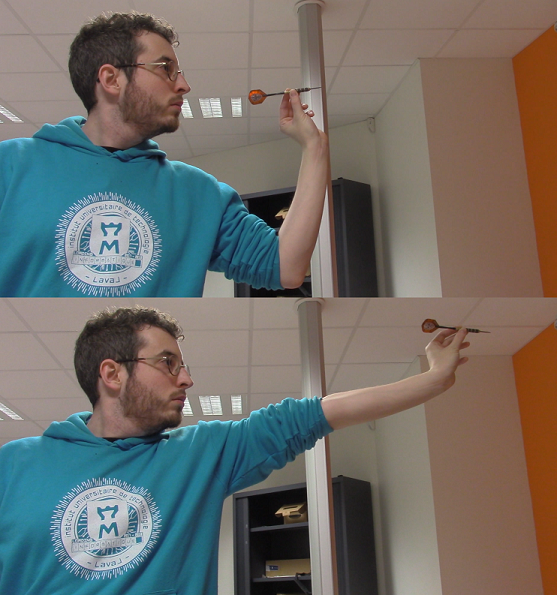
\includegraphics[scale=0.25]{img/darts_elbow_move_final.png}\\
				\\
				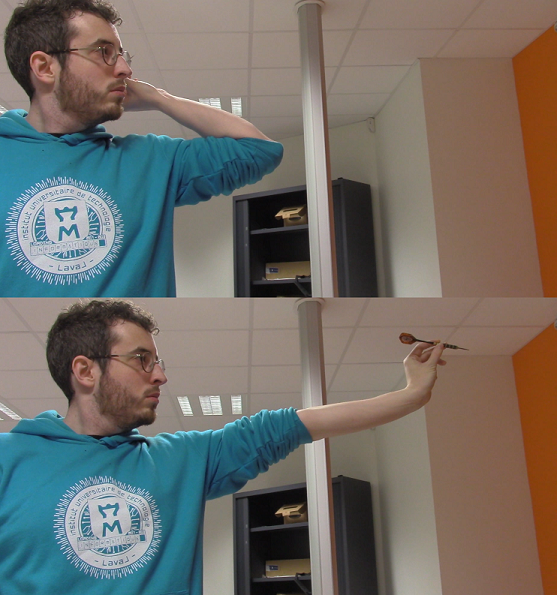
\includegraphics[scale=0.25]{img/darts_javelin_final.png} &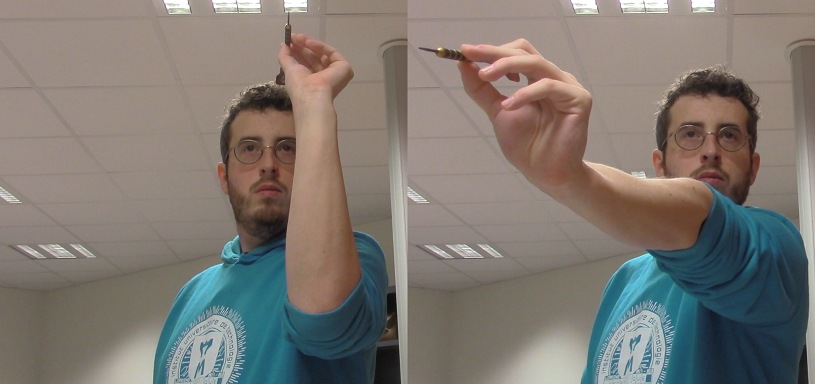
\includegraphics[scale=0.25]{img/darts_align_arm_final.png}\\
				Lancer type javelot (\textit{javelin)} & Alignement du bras (\textit{align arm})\\
			\end{tabular}}
		\end{table}
		
		

	\end{frame}
	
	\subsubsection{Données utilisées}
	\begin{frame}{\subsecname : \MakeLowercase{\subsubsecname}}
		\begin{block}{Descripteurs}
			\begin{itemize}[label=$\bullet$]
				\item \textit{Leaning} : vitesse moyenne des deux épaules
				\item \textit{Elbow move} : vitesse moyenne de coude et de l'épaule du côté de la préférence manuelle de la personne
				\item \textit{Javelin} : distance en x, y et z de la main par rapport à la tête
				\item \textit{Align arm} : moyenne de la largeur, ainsi que de l'écart-type, de la boîte englobante allant de la main à l'épaule du côté de la préférence manuelle de la personne
			\end{itemize}
		\end{block}
	\end{frame}
	
	\subsubsection{Déroulement}
	\begin{frame}{\subsecname : \MakeLowercase{\subsubsecname}}
		\begin{itemize}[label=$\bullet$]
			\item Pré-questionnaire : taille, niveau d'expertise auto-évalué aux fléchettes (échelle de Likert à 7 réponses), ainsi que toute pratique actuelle d'un sport
			\item Début de l'expérimentation
			\item 9 lancers, suivi de deux conseils, 4 fois d'affilée
			\item Post-questionnaire : ressenti de la personne par rapport à la combinaison, à la progression de son geste et à l'auto-évaluation de sa performance
		\end{itemize}
		
	\end{frame}
	
	\subsubsection{Résultats}
	\begin{frame}{\subsecname : \MakeLowercase{\subsubsecname}}
	Algorithme utilisé : k-means, avec $k=2$.
	
	\begin{table}[h]
		\centering
		\begin{tabular}{c|c|c}
			& \textit{Silhouette Score} &	 \textit{Adjusted Rand Index}\\\hline
			\textbf{\textit{Leaning}} & \cellcolor{green!25}0.85 & \cellcolor{green!25}1\\
			\textbf{\textit{Elbow move}} & \cellcolor{blue!25}0.58 & \cellcolor{yellow!25}0.47\\
			\textbf{\textit{Javelin}} & \cellcolor{green!25}0.79 & \cellcolor{green!25}1\\
			\textbf{\textit{Align arm}} & \cellcolor{blue!25}0.53 & \cellcolor{green!25}1\\
		\end{tabular}
	\end{table}
		
		Hypothèse \textbf{H3} validée dans le contexte de cette expérimentation
		
	\end{frame}
	
	\begin{frame}{\subsecname : \MakeLowercase{\subsubsecname}}
	Moyennes et écarts-types des données des apprenants (distance au centre de la cible) :
		\begin{table}[]
			\small
			
			\resizebox{\textwidth}{!}{%
			\begin{tabular}{l|llllllll}
 				& \multicolumn{2}{c}{\textbf{Série 1}} & \multicolumn{2}{c}{\textbf{Série 2}} & \multicolumn{2}{c}{\textbf{Série 3}} & \multicolumn{2}{c}{\textbf{Série 4}} \\
 				& \textit{Moyenne} & \textit{Écart-Type} & \textit{Moyenne} & \textit{Écart-Type} & \textit{Moyenne} & \textit{Écart-Type} & \textit{Moyenne} & \textit{Écart-Type} \\\hline
				\textbf{Groupe 1} & 10.15 & 3.83 & \cellcolor{red!25}14.42 & \cellcolor{red!25}5.47 & \cellcolor{orange!25}10.99 & \cellcolor{orange!25}3.27 & \cellcolor{yellow!25}10.25 & \cellcolor{yellow!25}3.60 \\
				\textbf{Groupe 2} & 10.25 & 3.70 & \cellcolor{red!25}13.57 & \cellcolor{red!25}6.45 & \cellcolor{orange!25}11.97 & \cellcolor{orange!25}4.61 & \cellcolor{yellow!25}10.93 & \cellcolor{yellow!25}3.66 \\
				\textbf{Groupe 3} & 9.74 & 2.30 & \cellcolor{red!25}11.97 & \cellcolor{red!25}4.06 & \cellcolor{orange!25}12.69 & \cellcolor{orange!25}5.73 & \cellcolor{yellow!25}11.01 & \cellcolor{yellow!25}5.45
			\end{tabular}}
		\end{table}
		
		\centering
		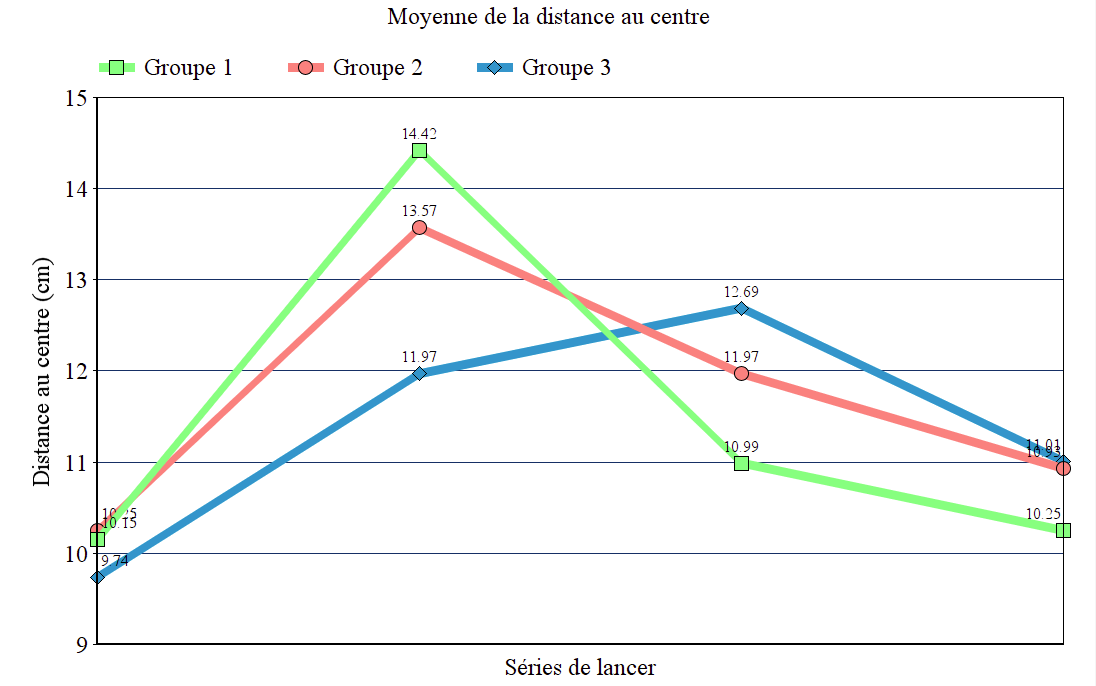
\includegraphics[scale=0.3]{img/moyenne_graphique.png}
	\end{frame}
	
	\begin{frame}{\subsecname : \MakeLowercase{\subsubsecname}}
		\begin{block}{Évaluation}
			Deux approches, en intergroupe et en intragroupe :
			\begin{itemize}[label=$\bullet$]
				\item Amélioration de l'objectif du mouvement (distance par rapport au centre de la cible)
				\item Amélioration des propriétés du mouvement (rapprochement du centroïde des données de l'apprenant au bon cluster de l'expert)
			\end{itemize}
		\end{block}
	\end{frame}
	
	\begin{frame}{\subsecname : \MakeLowercase{\subsubsecname}}
	
		En premier lieu, test de normalité : \textbf{Shapiro-Wilk} et \textbf{d'Agostino-Pearson}
		\begin{table}[]
			\begin{adjustbox}{max width=\textwidth}
			\begin{tabular}{l|l|l}
				\textit{Type de distribution} & \textit{Normale} & \textit{Non-normale} \\\hline
				\textbf{Intergroupe} & ANOVA & Kruskal-Wallis \\
 				& Levene & Wilcoxon-Mann-Whitney \\
 				& Student paire-à-paire &  \\\hline
				\textbf{Intragroupe} & Student sur deux échantillons & Rangs signés de Wilcoxon
			\end{tabular}
			\end{adjustbox}
		\end{table}
		
		\centering
		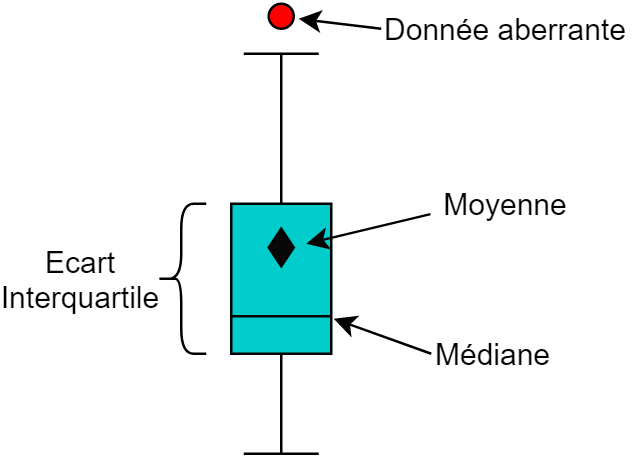
\includegraphics[scale=0.2]{img/boxplot.png}
	\end{frame}
	
	\begin{frame}{\subsecname : précision intergroupe}
		\centering
		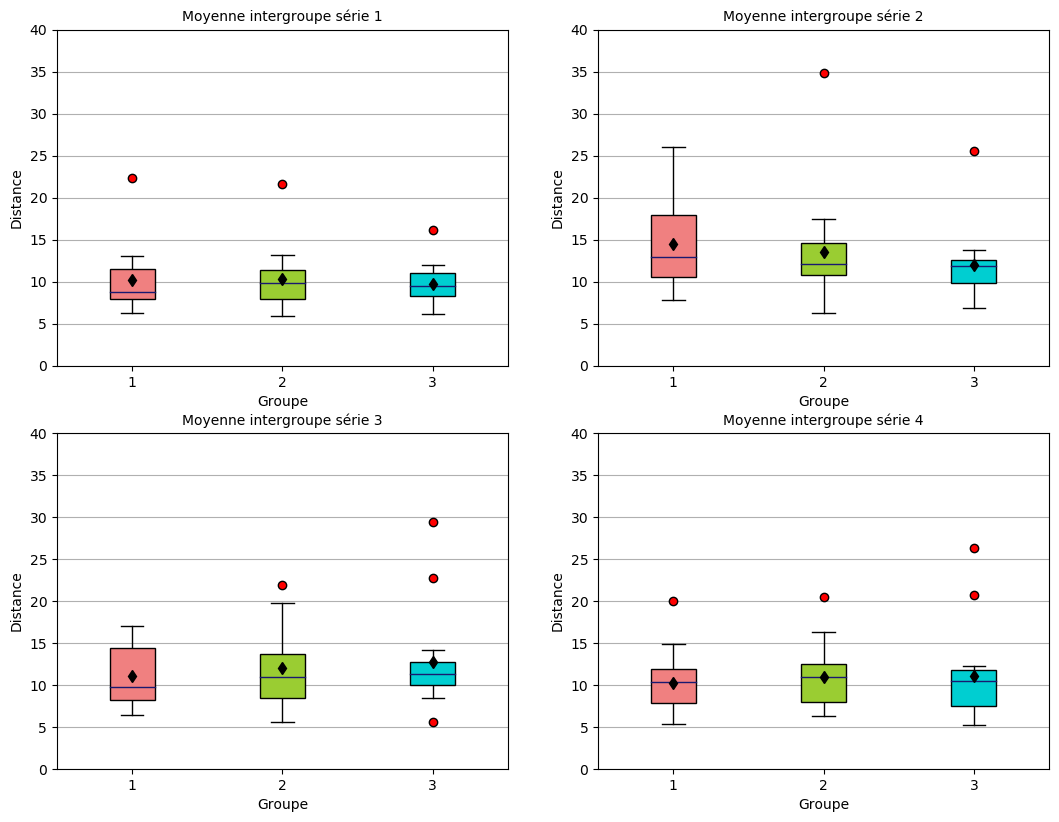
\includegraphics[scale=0.4]{img/Precision_All_data_intergroupe.png}
	\end{frame}
	
	\begin{frame}{\subsecname : précision intragroupe}
		\centering
		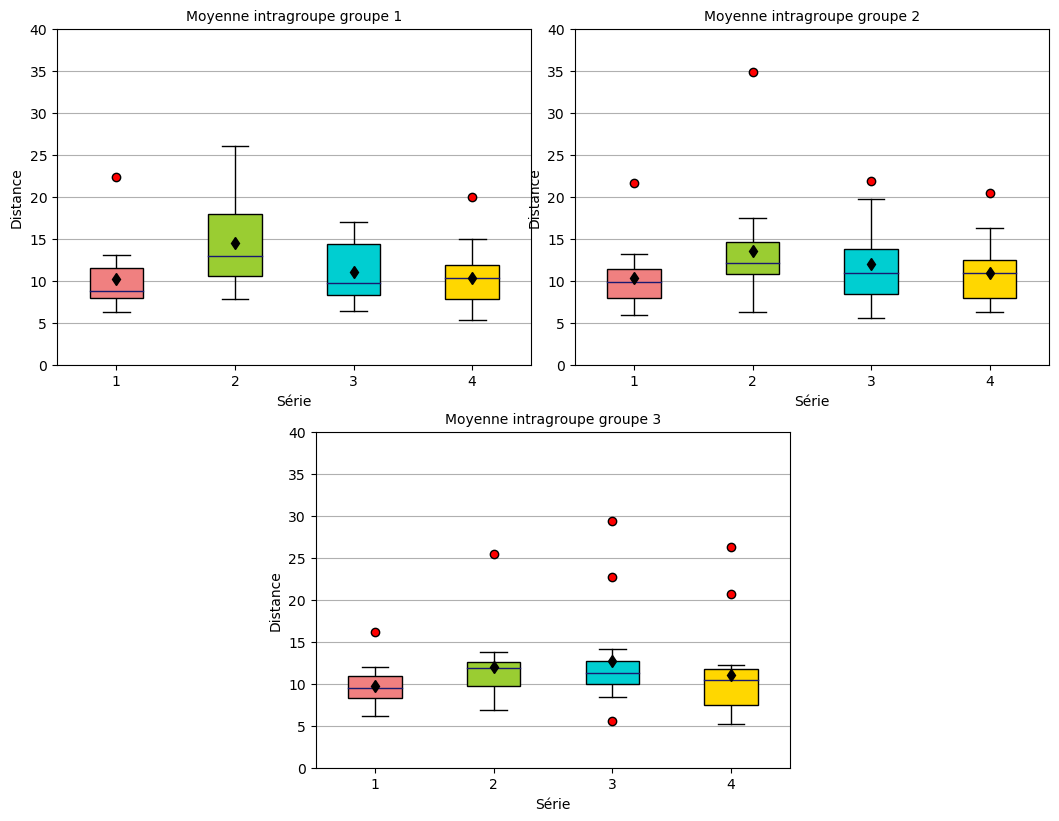
\includegraphics[scale=0.4]{img/Precision_All_data_intragroupe.png}
	\end{frame}
	
	\begin{frame}{\subsecname : \subsubsecname}
		Améliorations significatives en intragroupe entre les jeu 1 et 4 : \textit{leaning} et \textit{elbow move} pour tous les groupes, \textit{javelin} et \textit{align arm} pour le groupe 2 : \textbf{H4} est validée pour le groupe 2, et partiellement validée pour les autres groupes\\
		\vspace{1cm}
		Pas d'améliorations significatives en intergroupe : \textbf{H5} et \textbf{H6} ne sont pas validées
		
	\end{frame}
	
	\begin{frame}{\subsubsecname : questionnaires}
	\centering
		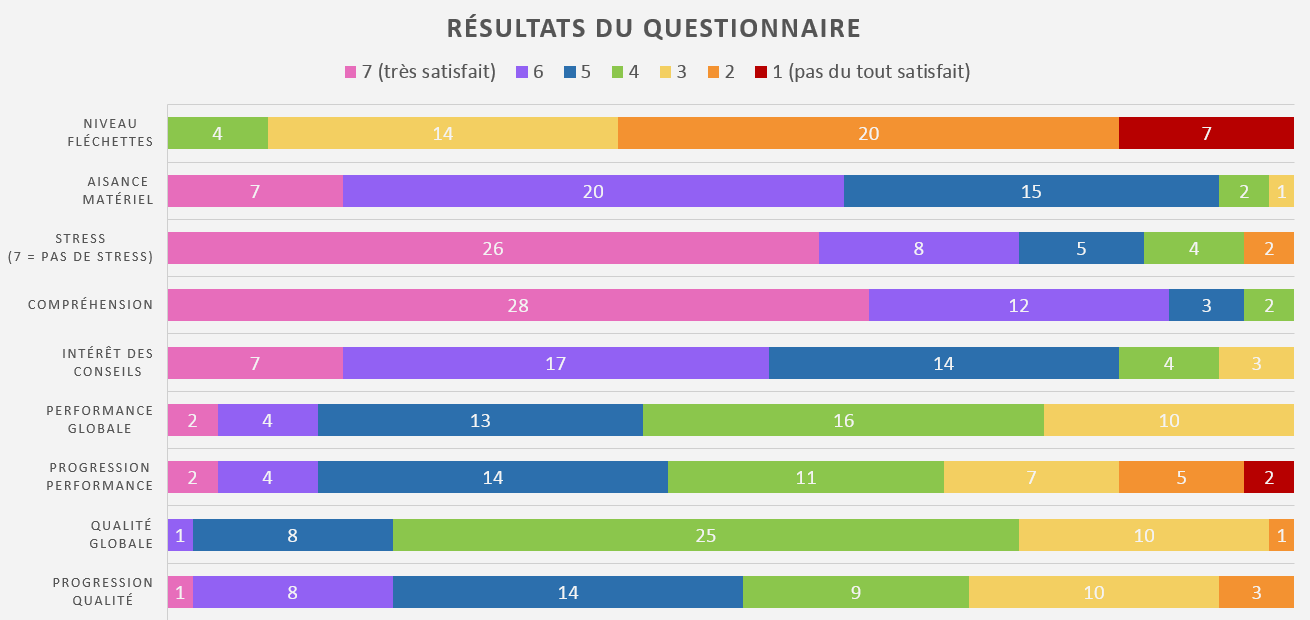
\includegraphics[scale=0.4]{img/graph_questionnaires.png}
	\end{frame}	
	
	\subsubsection{Limites}
	\begin{frame}{\subsecname : \MakeLowercase{\subsubsecname}}
		\begin{itemize}[label=$\bullet$]
			\item Phénomène d'auto-correction de l'expert
			\item Nombre de lancers pour les apprenants faibles (36)
			\item Pause entre chaque série de 9 lancers : perte du geste
			\item Systématiquement 2 conseils donnés
			\item Analyse de l'expert seul plus difficile dans le cadre de l'expérimentation
			\item Dans une situation d'apprentissage réelle, données extérieures au mouvement de l'apprenant
			\item L'évaluation du système suppose une prise en compte des conseils donnés
		\end{itemize}
	\end{frame}
	
	\section{Synthèse et perspectives}
	\subsection{Synthèse des contributions}
	
	\begin{frame}{\subsecname}
		\centering
		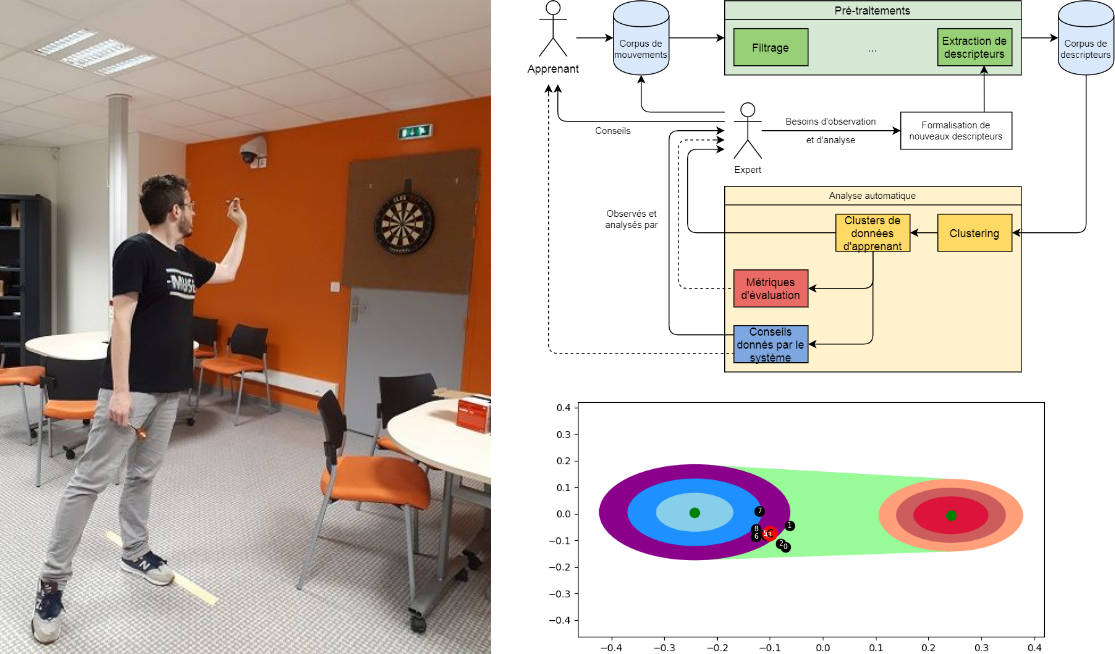
\includegraphics[scale=1.15]{img/resume.png}
	\end{frame}
	
	\subsection{Limites des travaux présentés}
	\begin{frame}{\subsecname}
		\begin{itemize}[label=$\bullet$]
			\item Techniques :
			\begin{itemize}[label=$-$]
				\item Manque d'interface graphique pour utiliser le système
				\item L'utilisation du Perception Neuron pour la captation implique l'utilisation de techniques de filtrage pour les données
			\end{itemize}
			
			\item Recherche :
			\begin{itemize}[label=$-$]
				\item Pertinence des indicateurs visuels à analyser
				\item Dans le cadre de l'expérimentation du lancer de fléchettes, faible nombre de lancers
			\end{itemize}
			
			
		\end{itemize}
	\end{frame}
	
	\subsection{Perspectives}
	\begin{frame}{\subsecname : explication des données non-alignées}
		Si dimensionnalité > 2, PCA : perte de sémantique
		
		\centering
			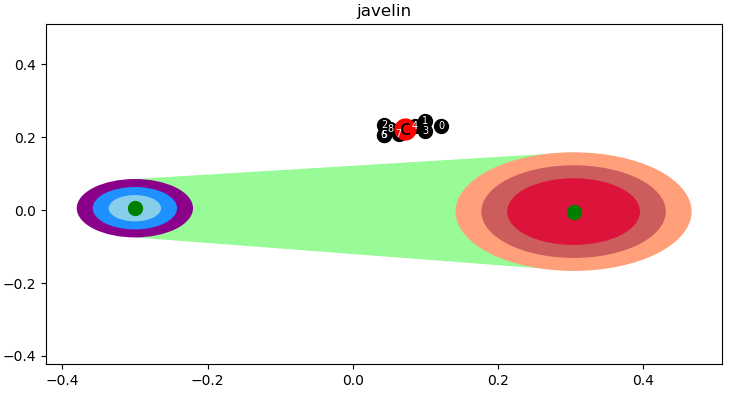
\includegraphics[scale=0.5]{img/non_aligned_default.png}
	\end{frame}
	
	\begin{frame}{\subsecname : création de nouveaux descripteurs}
		Système basé sur des patrons de conception :
		
		\begin{framed}
		DESCRIPTOR Hauteur hanche: POSITION\_ALL[2]
		\end{framed}
		pour la hauteur de la hanche (valeur en \textit{y}) calculée sur tout le mouvement\\

		\begin{framed}
		DESCRIPTOR Vitecceleration: SPEED\_ALL[2] + ACCELERATION\_ALL[1]
		\end{framed}
		pour calculer l'addition de la composante en $y$ de la vitesse et de la composante en $x$ de l'accélération\\
	\end{frame}
	
	\begin{frame}{\subsecname : clustering récursif}
		\begin{center}
			\includegraphics[scale=0.5]{img/subclustering/init2.png}
		\end{center}
		\begin{itemize}
			\item Clustering niveau 1 : vitesse du lancer
			\item Clustering niveau 2 : réussite du geste
		\end{itemize}
	\end{frame}
	
	\begin{frame}{Motion Learning Analytics}
		\centering
		\includegraphics[scale=1.15]{img/resume.png}
	\end{frame}


\end{document}







